\documentclass[11pt]{article}

% MSOM e-companion: separate document, <=16 pages, sections labeled EC.1, EC.2, ...
\usepackage[margin=1in]{geometry}
\usepackage{setspace}
\doublespacing
\emergencystretch 3em

\usepackage{graphicx}
% Prefer vector art: figures are included without an extension so LaTeX picks
% the PDF when one exists and falls back to the raster preview otherwise.
% INFORMS requires vector PDF/EPS for plots (style instructions Sec. 9.1);
% only genuine images (the hand-drawn logistics diagram) stay raster.
\DeclareGraphicsExtensions{.pdf,.png,.jpg,.jpeg}
\usepackage{float}
\usepackage{subcaption}
\usepackage{amsmath,amssymb,amsthm,enumitem,mathtools}
\renewcommand{\qedsymbol}{$\blacksquare$}
\usepackage{booktabs}
\usepackage{multirow}
\usepackage[round,authoryear]{natbib}
\bibliographystyle{plainnat}
\usepackage[colorlinks=true, citecolor=blue, linkcolor=blue, urlcolor=blue]{hyperref}
\usepackage[acronyms]{glossaries}
\makeglossaries
\usepackage{xcolor}
\input{definitions.tex}

% EC section / equation / figure / table numbering
\renewcommand{\thesection}{EC.\arabic{section}}
\renewcommand{\theequation}{EC.\arabic{equation}}
\renewcommand{\thefigure}{EC.\arabic{figure}}
\renewcommand{\thetable}{EC.\arabic{table}}
\renewcommand{\thetheorem}{EC.\arabic{theorem}}
\renewcommand{\theproposition}{EC.\arabic{proposition}}
\renewcommand{\thelemma}{EC.\arabic{lemma}}

\title{\textbf{E-Companion:\\ Robust Antimicrobial Supply Chain Design under\\ Epidemiological Demand Uncertainty in Botswana}}
\date{}

\begin{document}
\maketitle
\vspace{-3em}
\begin{center}
\textit{This e-companion collects the dualization derivation, proofs, the epidemic model, and extended sensitivity analyses referenced in the main text.}
\end{center}
\bigskip

% ======================= EC.1 DUALIZATION =======================
\section{Dualization: Proof of Proposition~1}
\label{ec:dualization}

We derive the tractable single-level reformulation of the affinely-adjustable robust problem, establishing Proposition~1 of the main text.
Throughout, the affine decision rule is $F_{(u,v),k}^{(t)}(\xi) = \bar F_{(u,v),k}^{(t)} + \alpha_{(u,v),k}^{(t)}\,\xi_{v,k}^{(t)}$, and the uncertainty set is the budgeted set $\mathcal{U}^{(k)}$.

\subsection{Robust feasibility conditions}

\emph{Inventory balance.}
Substituting the affine rule into the inventory balance and collecting the terms in $\xi$, the uncertain component at node $n$ is
\begin{equation}
\Big(\textstyle\sum_{j:(j,n)\in A}\alpha_{(j,n),k}^{(t)} - 1\Big)\xi_{n,k}^{(t)}
- \sum_{r:(n,r)\in A}\alpha_{(n,r),k}^{(t)}\xi_{r,k}^{(t)}.
\end{equation}
Robust feasibility requires that its worst case over $\mathcal{U}^{(k)}$ not exceed the deterministic slack:
\begin{align}
\max_{\xi\in\mathcal{U}^{(k)}}\Big[\Big(\textstyle\sum_{j:(j,n)\in A}\alpha_{(j,n),k}^{(t)} - 1\Big)\xi_{n,k}^{(t)}
- \sum_{r:(n,r)\in A}\alpha_{(n,r),k}^{(t)}\xi_{r,k}^{(t)}\Big]
\le\;& I_{n,k}^{(t+1)} - I_{n,k}^{(t)}
- \textstyle\sum_{j:(j,n)\in A}\bar F_{(j,n),k}^{(t)} \notag\\
& + \textstyle\sum_{r:(n,r)\in A}\bar F_{(n,r),k}^{(t)}
- \mathbf{1}_{\{n=0\}}q_k^{(t)}
+ \bar D_{n,k}^{(t)} - U_{n,k}^{(t)}.
\label{eq:ec-inv-robust}
\end{align}

\emph{Availability and capacity.}
The same substitution into the shipment-availability constraint of the main text and the arc-capacity constraint yields uncertain components
\begin{equation}
\textstyle\sum_{r:(n,r)\in A}\alpha_{(n,r),k}^{(t)}\xi_{r,k}^{(t)} - \Big(\sum_{j:(j,n)\in A}\alpha_{(j,n),k}^{(t)}\Big)\xi_{n,k}^{(t)}
\quad\text{and}\quad
\textstyle\sum_{k}\alpha_{(i,j),k}^{(t)}\xi_{j,k}^{(t)},
\end{equation}
respectively, each of which must satisfy an analogous worst-case-$\le$-slack condition.

\subsection{Dualizing the inner maximization}

Using the Bertsimas--Sim representation $\xi_{r,k}^{(t)} = \sigma_{r,k}^{(t)}(z_{r,k}^{+} - z_{r,k}^{-})$ with $0 \le z_{r,k}^{\pm}\le 1$ and $\sum_r (z_{r,k}^{+}+z_{r,k}^{-})\le\Gamma$, each inner maximization is a linear program in $(z^{+},z^{-})$.
Taking its linear-programming dual replaces the maximization by a minimization over nonnegative multipliers, and because the outer problem minimizes, the two combine into a single minimization.
For the inventory constraint we introduce a budget multiplier $\theta_{n,k}^{(t)}$ and per-node deviation multipliers $\pi_{n,k,r}^{\pm(t)}$, giving the finite system
\begin{align}
\Gamma\,\theta_{n,k}^{(t)} + \textstyle\sum_{r\in R(n)}\big(\pi_{n,k,r}^{+(t)}+\pi_{n,k,r}^{-(t)}\big)
\;\le\;& I_{n,k}^{(t+1)} - I_{n,k}^{(t)}
- \textstyle\sum_{j:(j,n)\in A}\bar F_{(j,n),k}^{(t)}
+ \sum_{r:(n,r)\in A}\bar F_{(n,r),k}^{(t)} \notag\\
& - \mathbf{1}_{\{n=0\}}q_k^{(t)} + \bar D_{n,k}^{(t)} - U_{n,k}^{(t)}, \\
\theta_{n,k}^{(t)} + \pi_{n,k,n}^{+(t)} \;\ge\;& \Big(\textstyle\sum_{j:(j,n)\in A}\alpha_{(j,n),k}^{(t)}-1\Big)\sigma_{n,k}^{(t)}, \\
\theta_{n,k}^{(t)} + \pi_{n,k,n}^{-(t)} \;\ge\;& -\Big(\textstyle\sum_{j:(j,n)\in A}\alpha_{(j,n),k}^{(t)}-1\Big)\sigma_{n,k}^{(t)},
\end{align}
together with the analogous inequalities for each $r$ with $(n,r)\in A$, all multipliers nonnegative.
Here $R(n) = \{n\}\cup\{r : (n,r)\in A\}$ collects the node itself and its downstream neighbours, which are the only deviations entering the constraint; multipliers for other nodes would be identically zero and are not introduced.
The availability and arc-capacity constraints dualize identically, introducing multipliers $(\tilde\theta,\tilde\pi^{\pm})$ and $(\eta,\rho^{\pm})$ respectively; the resulting inequalities have the same structure and are omitted for brevity.

\subsection{Conclusion of the proof}

Each robust constraint has been replaced by finitely many linear inequalities in the original variables $(\bar F,\alpha,I,U,q,\lambda,y)$ and the nonnegative multipliers $(\theta,\pi^{\pm},\tilde\theta,\tilde\pi^{\pm},\eta,\rho^{\pm})$.
The inventory and availability constraints introduce one budget multiplier per node--class and one deviation multiplier pair per element of $R(n)$, and the capacity constraints introduce one multiplier pair per arc--class, so the reformulation adds $O(|N|K + |A|K)$ variables and constraints.
The adjustable robust allocation problem is therefore an exact single-level mixed-integer linear program of size linear in $|N|$, $|A|$, and $K$, which proves Proposition~1. \hfill$\blacksquare$

% ======================= EC.2 PROOFS =======================
\section{Proofs for the Demand Estimator}
\label{ec:proofs}

\begin{lemma}[Smoothness of the demand map]
\label{lem:smooth}
The map $g(\beta) = \sum_a N_{r,a}\,\delta_a\exp(x_{r,a}^{T}\beta)$ is twice continuously differentiable and Lipschitz on compact subsets of $\reals^{d}$.
\end{lemma}
\begin{proof}
Each summand is a fixed positive constant times $\exp(x_{r,a}^{T}\beta)$, a smooth function of $\beta$ composed with a linear map, and finite sums of smooth functions are smooth, so $g$ is twice continuously differentiable.
Its gradient $\nabla g(\beta) = \sum_a N_{r,a}\,\delta_a\,x_{r,a}\exp(x_{r,a}^{T}\beta)$ is continuous, hence bounded on any compact set by some $L$, and the mean value theorem gives $|g(\beta_1)-g(\beta_2)|\le L\|\beta_1-\beta_2\|$.
\end{proof}

\noindent\textit{Proof of Proposition~2 (consistency).}
Under the negative-binomial generalized-linear-model assumptions and standard regularity conditions, maximum likelihood is consistent, $\hat\beta_n \to \beta^{\star}$ in probability.
By Lemma~\ref{lem:smooth} the map $g$ is continuous, so the continuous mapping theorem gives $\hat D_r = g(\hat\beta_n) \to g(\beta^{\star}) = D_r^{\star}$ in probability. \hfill$\blacksquare$

\medskip
\noindent\textit{Proof of Proposition~3 (dependence-preserving aggregation).}
By linearity of expectation, $\mathbb{E}[D_i] = \sum_{j=1}^{N}\mathbb{E}[Y_{j,i}]$, and identical distribution across patients gives $\mathbb{E}[D_i] = N\,\mathbb{E}[Y_{1,i}]$.
For the covariance, $\mathrm{Cov}(D_i,D_{i'}) = \sum_{j}\sum_{\ell}\mathrm{Cov}(Y_{j,i},Y_{\ell,i'})$; independence across patients kills the $j\neq\ell$ terms, leaving $\sum_j \mathrm{Cov}(Y_{j,i},Y_{j,i'}) = N\,\mathrm{Cov}(Y_{1,i},Y_{1,i'})$, which is unrestricted.
Thus aggregation preserves marginal means while permitting arbitrary within-patient dependence across classes. \hfill$\blacksquare$

% ======================= EC.3 EPIDEMIC MODEL =======================
\section{The Epidemic Coupling}
\label{ec:seir}

We give the two-strain model used in the epidemic-driven extension.
The hospital population is partitioned into susceptible $S$, exposed and infectious for the drug-susceptible strain $E_s,I_s$, exposed and infectious for the drug-resistant strain $E_r,I_r$, and recovered $R$, with $N=S+E_s+I_s+E_r+I_r+R$.
Forces of infection are $\lambda_s = \beta_s I_s/N$ and $\lambda_r = \beta_r I_r/N$, with $\beta_r = 0.8\,\beta_s$ a fitness cost.
The dynamics are
\begin{align}
\dot S &= \mu N - (\lambda_s+\lambda_r)S - \mu S, &
\dot E_s &= \lambda_s S - (\sigma_s+\mu)E_s, \notag\\
\dot I_s &= \sigma_s E_s - (\tau_s+\gamma_s+\mu)I_s, &
\dot E_r &= \lambda_r S + \rho\,\tau_s I_s - (\sigma_r+\mu)E_r, \notag\\
\dot I_r &= \sigma_r E_r - (\tau_r+\gamma_r+\mu)I_r, &
\dot R &= \gamma_s I_s + \gamma_r I_r + (1-\rho)\tau_s I_s + \tau_r I_r - \mu R.
\end{align}
The amplification probability $\rho$ is the fraction of treated susceptible infections that convert to resistant rather than recovering.
The coupling to the supply chain enters through the treatment rates,
\begin{equation}
\tau_s = \tau_s^{0}\min\!\Big(\tfrac{a_1}{a_1^{\star}},1\Big), \qquad
\tau_r = \tau_r^{0}\min\!\Big(\tfrac{a_2}{a_2^{\star}},1\Big),
\end{equation}
where $a_1,a_2$ are the realized supply rates of cephalosporins and carbapenems and $a_1^{\star},a_2^{\star}$ their nominal levels from the MDE, so a stockout depresses treatment and, through the $\rho\tau_s I_s$ term, feeds resistance.

The system is integrated in closed loop with the allocation model.
Writing $y^{(t)}$ for the compartment vector at the start of period $t$, one period proceeds as follows.
Demand for cephalosporins and carbapenems at the hospital is set from the current infectious populations, $\bar D^{(t)}_{\text{ceph}} = \tau_s^{0} I_s^{(t)}\Delta t$ and $\bar D^{(t)}_{\text{carb}} = \tau_r^{0} I_r^{(t)}\Delta t$ with $\Delta t$ the period length.
The allocation problem is solved for that demand, starting from the inventory carried out of period $t-1$, and we record the quantities $a_1^{(t)}, a_2^{(t)}$ actually delivered.
The compartmental system is then advanced over $\Delta t$ with treatment rates evaluated at that realized supply, giving $y^{(t+1)}$, from which the next period's demand follows.
Because the demand a policy faces in period $t+1$ depends on what it failed to deliver in period $t$, the two systems co-evolve rather than being coupled only through a post-hoc comparison.
Parameters are calibrated to gram-negative infection dynamics at Princess Marina Hospital and to Botswana treatment-coverage data, with several biological rates taken from \citet{kd20}; we regard the calibration as illustrative.

\paragraph{Two-year resistance dynamics.}
Over the two-year horizon of the main-text extension, supply performance measurably affects both infectious compartments (Figure~\ref{fig:resistance}).
Under the deterministic policy, chronic cephalosporin shortages suppress $\tau_s$, slowing clearance of the susceptible strain and sustaining the amplification pathway at elevated levels; the two robust policies clear both strains faster.
Static robust and ARO-ADR are nearly indistinguishable here, consistent with the weak amplification channel ($\rho = 0.07$) over a two-year window.

\begin{figure}[H]
    \centering
    
\includegraphics[width=0.95\linewidth]{figures/resistance_emergence_comparison}
    \caption{Resistance and susceptible-strain dynamics at Princess Marina Hospital over two years. \textbf{Left:} drug-resistant infectious population $I_r$. \textbf{Right:} drug-susceptible infectious population $I_s$. The deterministic policy clears both strains more slowly than the robust policies.}
    \label{fig:resistance}
\end{figure}

\paragraph{Long-horizon behavior.}
Extending the integration to 50 years under each policy's steady coverage (Figure~\ref{fig:seirlong}) shows the resistant \emph{fraction} $I_r/(I_s+I_r)$ remaining marginally higher under better-supplied policies at every horizon, without reversing, while the absolute resistant burden $I_r$ is lower under ARO-ADR throughout the policy-relevant range.
The higher fraction is a denominator effect of faster susceptible-strain clearance, not evidence of greater resistance emergence, which is why we read the framework's benefits as coverage rather than resistance effects.

\begin{figure}[H]
    \centering
    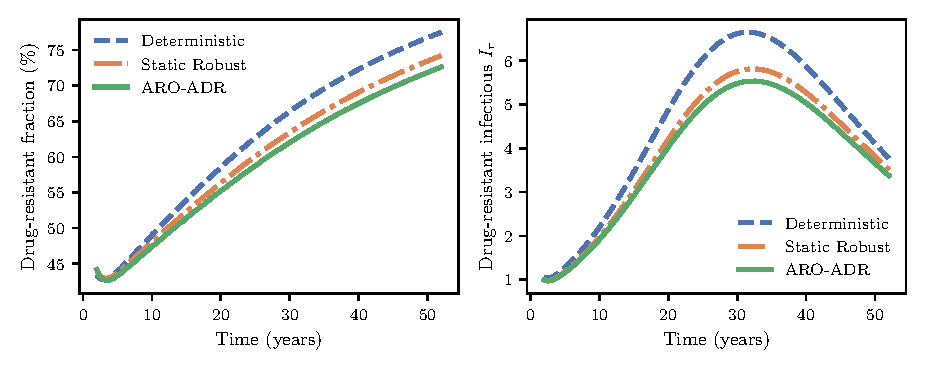
\includegraphics[width=0.95\linewidth]{figures/seir_resistance_longhorizon}
    \caption{Two-strain SEIR extended to a 50-year horizon under each policy's steady supply coverage. \textbf{Left:} the resistant fraction $I_r/(I_s+I_r)$ stays marginally higher under better-supplied policies and does not reverse. \textbf{Right:} absolute resistant burden $I_r$ is lower under ARO-ADR throughout.}
    \label{fig:seirlong}
\end{figure}

% ======================= EC.4 EXTENDED SENSITIVITY =======================
\section{Extended Sensitivity Analyses}
\label{ec:sensitivity}

\paragraph{Uncertainty budget.}
Figure~\ref{fig:gamma} varies the budget $\Gamma$ across dispersion levels.
The ARO-ADR advantage over static robust is largest at small $\Gamma$ and high variability and vanishes as $\Gamma$ grows, since a large budget forces worst-casing over many nodes and suppresses the adaptive component, collapsing ARO-ADR toward the static policy.

\begin{figure}[H]
    \centering
    
\includegraphics[width=0.95\linewidth]{figures/gamma_sensitivity}
    \caption{Realized unmet demand (\%) across policies for varying uncertainty budget $\Gamma$ (columns) and dispersion $\kappa$ (rows). ARO-ADR converges to static robust as $\Gamma$ grows.}
    \label{fig:gamma}
\end{figure}

\paragraph{Shortage penalty.}
Figure~\ref{fig:penalty} varies the per-unit shortage penalty at fixed unit procurement cost.
Below the procurement cost, serving demand is not cost-effective and unmet demand rises sharply; above it, realized unmet demand saturates and is essentially invariant to the penalty, because achievable service is pinned by physical capacity and the uncertainty set.
The operationally relevant regime, where clinical stockout costs far exceed procurement, is the saturated one.

\begin{figure}[H]
    \centering
    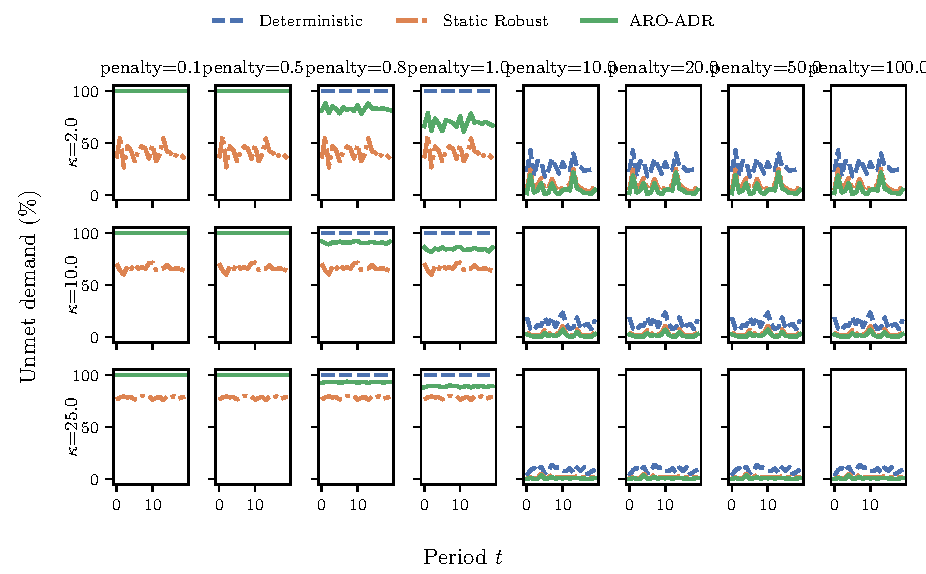
\includegraphics[width=0.95\linewidth]{figures/penalty_sensitivity}
    \caption{Realized unmet demand (\%) across policies for varying shortage penalty (columns; unit procurement cost $1$) and dispersion $\kappa$ (rows). Above the procurement cost, unmet demand saturates and the policy ordering is insensitive to the penalty.}
    \label{fig:penalty}
\end{figure}

\paragraph{Seasonal (non-stationary) demand.}
As a further robustness check we impose a seasonal demand multiplier calibrated to documented tuberculosis-diagnosis seasonality in Southern Africa \citep{ballif2018}, so that the mean demand varies over a two-cycle horizon.
When the optimizer is given only stationary forecasts, all policies suffer unmet-demand spikes above 50\% at the seasonal peaks; when it is given the seasonally-adjusted means, ARO-ADR attains a mean unmet rate of $0.72\%$, against $2.21\%$ for static robust and $8.39\%$ for deterministic (Figure~\ref{fig:seasonal}).
The check confirms the policy ordering is preserved under structured non-stationarity, not only i.i.d.\ variation.

\begin{figure}[H]
    \centering
    \begin{subfigure}[b]{0.48\textwidth}
        \centering
\includegraphics[width=\textwidth]{figures/seasonal_unmet_no_multiplier}
        \caption{Stationary forecast supplied.}
    \end{subfigure}\hfill
    \begin{subfigure}[b]{0.48\textwidth}
        \centering
\includegraphics[width=\textwidth]{figures/seasonal_unmet_with_multiplier}
        \caption{Seasonally-adjusted forecast supplied.}
    \end{subfigure}
    \caption{Realized unmet demand over two seasonal cycles. Supplying the seasonally-adjusted mean lets all policies pre-position ahead of peaks; ARO-ADR benefits most. Curves are means over 12 independent demand realizations; bands are $95\%$ confidence intervals.}
    \label{fig:seasonal}
\end{figure}

\paragraph{Disaggregated cost maps.}
Figures~\ref{fig:cmsfull2526} and~\ref{fig:cmsfull2627} decompose the real-CMS results of the main text (Section~6.3) by cost component and district, for the 2025--26 and 2026--27 scenarios.
The higher objective under the deterministic policy is driven primarily by shortage cost rather than procurement or transport; procurement cost is broadly uniform across districts within each policy; and holding cost rises under the robust policies as they pre-position inventory to hedge, the mechanism through which they improve service.
Kweneng is a persistent transport-cost outlier, reflecting its geographic size.
Figure~\ref{fig:natmaps} gives the analogous decomposition for the national simulation.

\begin{figure}[H]
    \centering
    
\includegraphics[width=0.702\textwidth]{figures/cms_full_metrics_2526}
    \caption{Real CMS data, 2025--26 scenario: district-level maps of average unmet demand, objective, procurement, transport, holding, and shortage cost (rows) under the three policies (columns). District names are omitted at this panel size; the geography is identical in every panel and is labelled in the main text.}
    \label{fig:cmsfull2526}
\end{figure}

\begin{figure}[H]
    \centering
    
\includegraphics[width=0.702\textwidth]{figures/cms_full_metrics_2627}
    \caption{Real CMS data, 2026--27 scenario: layout as in Figure~\ref{fig:cmsfull2526}.}
    \label{fig:cmsfull2627}
\end{figure}

\begin{figure}[H]
    \centering
    
\includegraphics[width=0.702\textwidth]{figures/botswana_appendix_simulation_maps}
    \caption{National simulation: district-level maps of each cost component under the three policies. District names are omitted at this panel size; the geography is identical in every panel and is labelled in the main text.}
    \label{fig:natmaps}
\end{figure}

\bibliography{bibliography}

\end{document}
